
\subsection{Application} \label{application}

The application for this project has been implemented as a custom single-page web application using Vite \cite{viteDocs}, React \cite{reactDocs} and React Router \cite{reactRouterDocs}. It offers an interactive map and results table which dynamically update based on a number of different configurations options provided to the user. To obtain the results of the queries, the application connects to the running Ontop system via its SPARQL \cite{hogan2020sparql} endpoint.

\begin{figure}[ht!]
    \centering
    \hfill
    \begin{subfigure}[t]{0.48\linewidth}
        \centering
        
\includegraphics[width=\linewidth]{figures/home.png}
        \caption{Example screenshot of the landing page of the application. In the very center of the page there is a search bar with which the user can select one of the predefined configurations.}
        \label{fig:home}
    \end{subfigure}
    \hfill
    \begin{subfigure}[t]{0.48\linewidth}
        \centering
        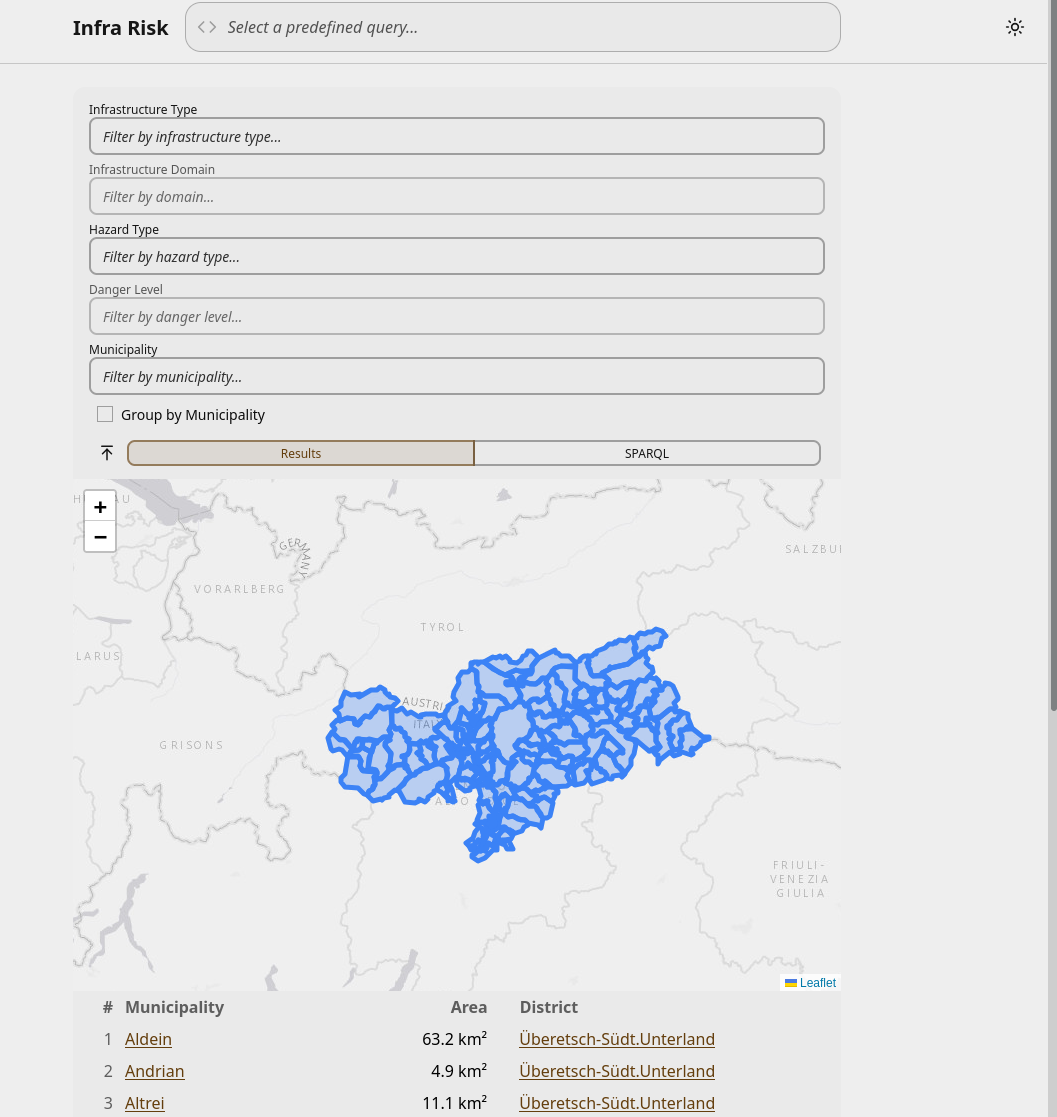
\includegraphics[width=\linewidth]{figures/municipalities.png}
        \caption{Example screenshot of the application returning the result for a simple query listing all municipalities in the knowledge graph. Below the header, which contains the search bar for selecting other predefined queries, the application lists a number of configuration options to customize the query.}
        \label{fig:municipalities}
    \end{subfigure}
    \hfill
    \caption{Example screenshot extracted from the application showing how it can be configured manually or using predefined queries.}
    \label{fig:example1}
\end{figure}

The main SPARQL query used for with the Ontop endpoint is generated dynamically based on the configurations made by the user. A small number of queries has been predefined, each serving as the answer to a concrete question related to the chosen domain. Note that these are simply configuring the exact same options that are also made available directly to the user, and do not include any special cases. \Cref{fig:home} shows how these can be selected from the home screen of the application. When inside any other screen, the predefined queries can still be accessed easily with the search bar located in the application header.

However, it is not necessary to restrict oneself to the predefined queries. \Cref{fig:municipalities} show the set of available configurable values. The first option field allows selecting the type of infrastructure to consider, lines or nodes. The second relates to the infrastructure domain, possibly filtering based on water, energy, waste, communication, or electricity related assets. Similarly to the infrastructure, also the hazards have a configurable field for whether to include avalanches, landslides, both, or neither. For the hazard zones a fourth configuration field allows selecting the danger levels to consider in the queries. Finally, it is possible to configure only a subset of municipalities to analyze, and optionally to aggregate the result by municipality. The latter is useful for answering questions about the number of vulnerable infrastructure assert per municipality. Taken together these configuration options are sufficient to implement all four example application questions that have been formulated in \cref{into} of the report. For example, by not selecting any hazard type, the query is transformed into one that returns all infrastructure assets regardless of exposure. Similarly by not selecting any infrastructure type, the query is adapted to one that instead searches for hazard zones instead of infrastructure types. Removing all types for both infrastructure and hazard results in a query simply retrieving all municipalities, corresponding to what is shown in \cref{fig:municipalities}. As soon as the user modifies some options, a new query is generated from it and executed against the Ontop endpoint to update the user interface as soon as the results have been received. A loading animation is shown while the application awaits the reception of the results to the latest query.

\begin{figure}[ht!]
    \centering
    \hfill
    \begin{subfigure}[t]{0.48\linewidth}
        \centering
        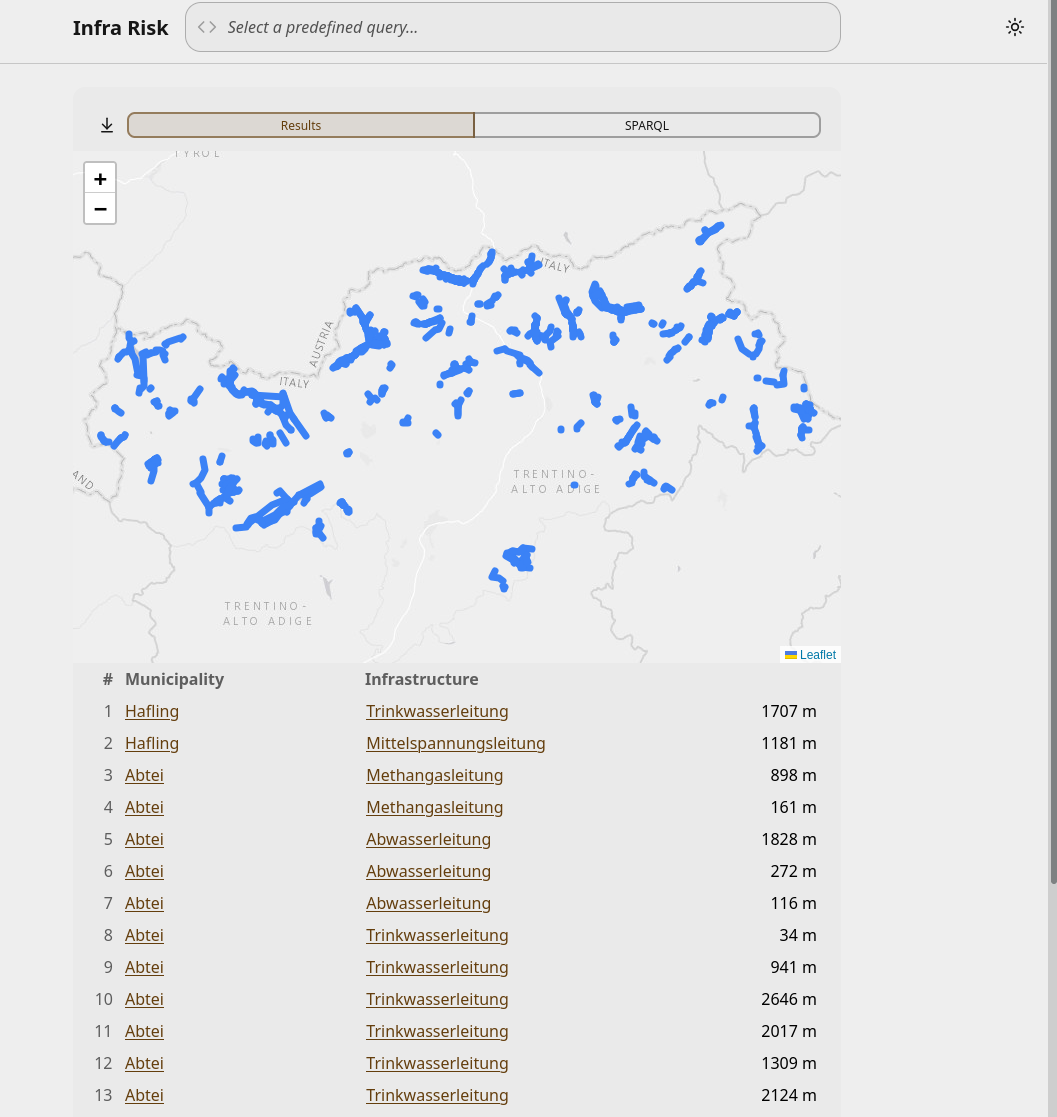
\includegraphics[width=\linewidth]{figures/avalanche.png}
        \caption{Screenshot of the application showing the results for a more complicated query involving the discovery of vulnerable infrastructure lines. The results of the currently configured query are displayed both as a map and as a table.}
        \label{fig:avalanche}
    \end{subfigure}
    \hfill
    \begin{subfigure}[t]{0.48\linewidth}
        \centering
        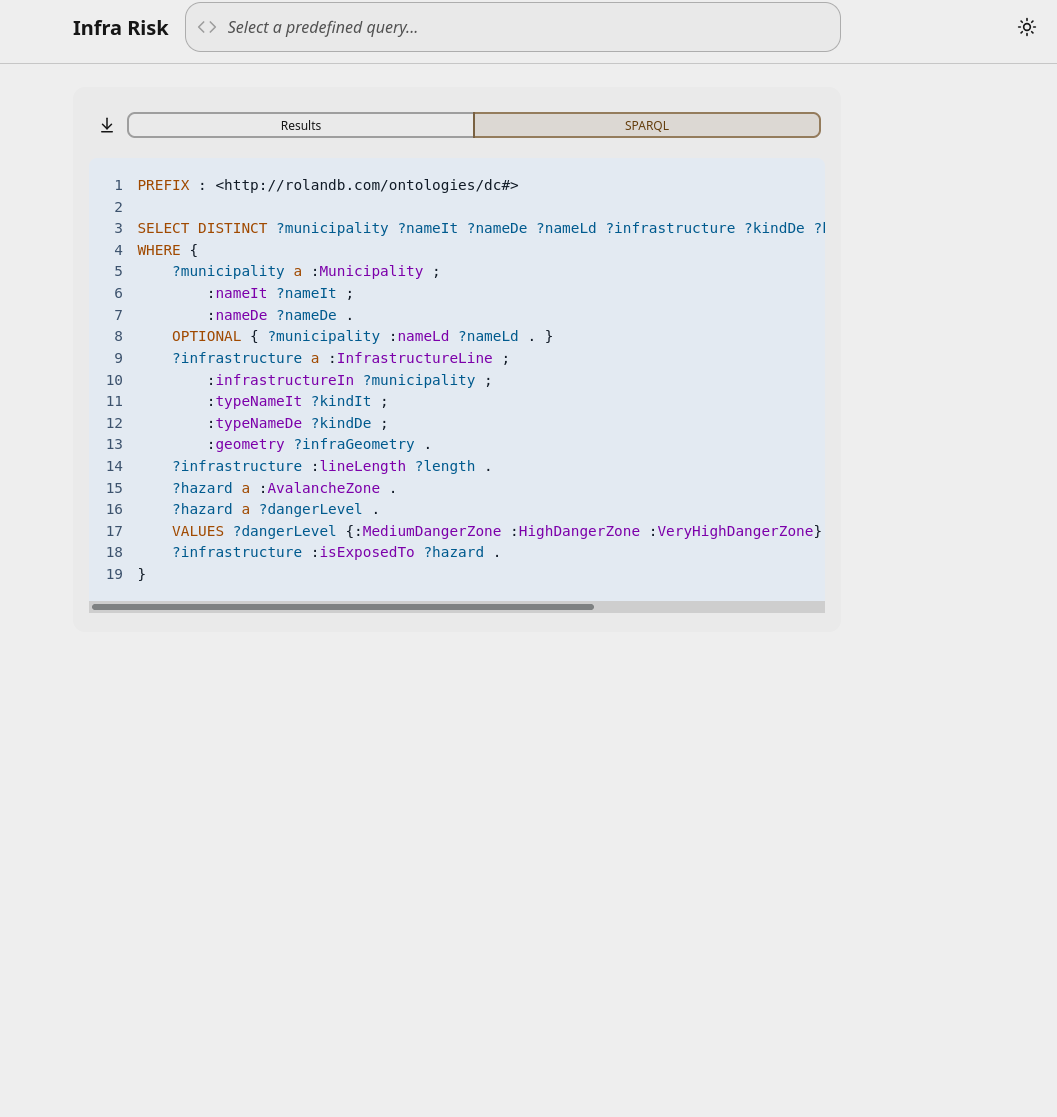
\includegraphics[width=\linewidth]{figures/sparql.png}
        \caption{Screenshot of the application showing the ability to display the SPARQL query that is being used to retrieve the results given the current configuration of the application.}
        \label{fig:sparql}
    \end{subfigure}
    \hfill
    \caption{Example screenshot extracted from the application showing how results are displayed.}
    \label{fig:example2}
\end{figure}



\begin{figure}[ht!]
    \centering
    \hfill
    \begin{subfigure}[t]{0.48\linewidth}
        \centering
        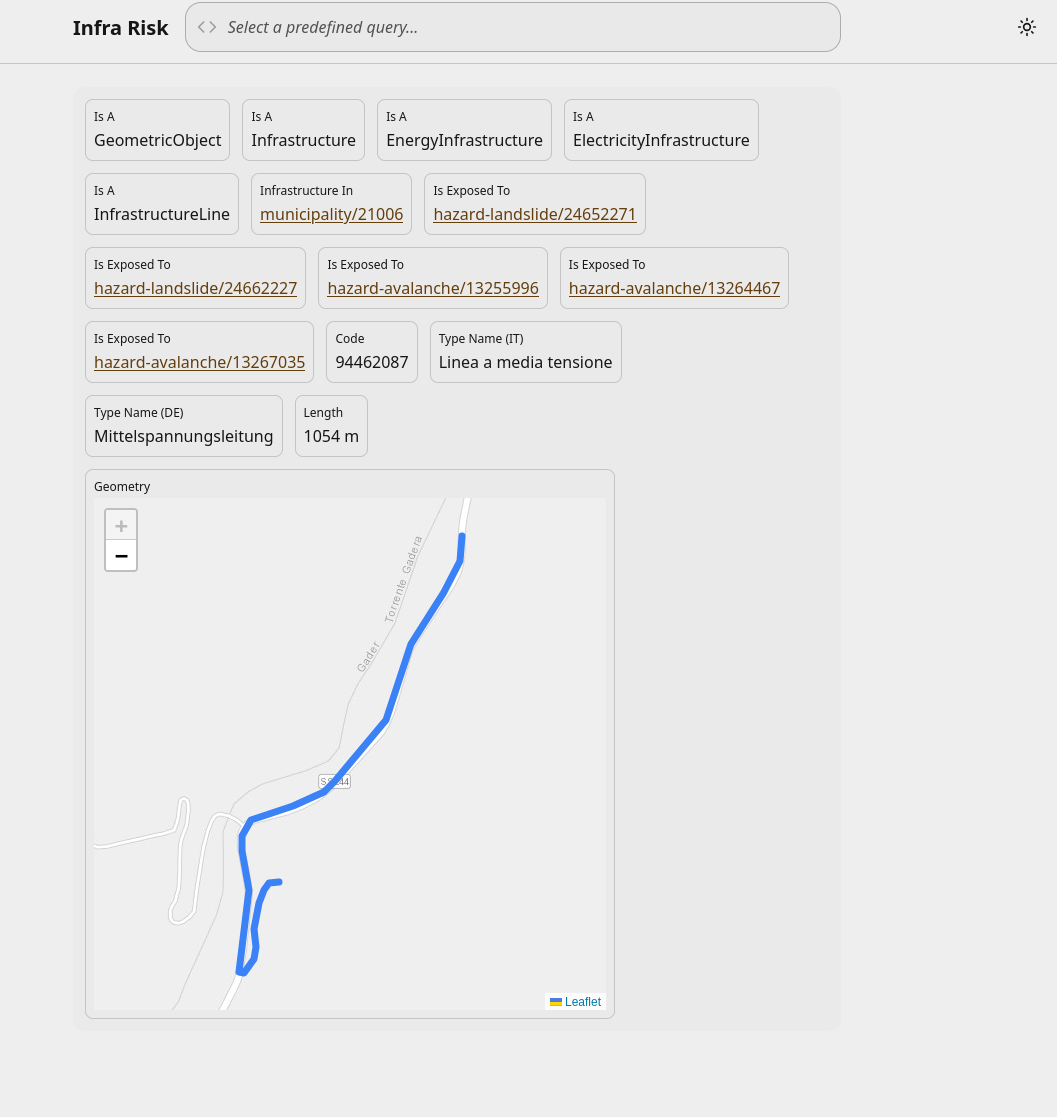
\includegraphics[width=\linewidth]{figures/infrastructure.png}
        \caption{Application screenshot that shows details regarding one specific infrastructure line.}
        \label{fig:infrastructure}
    \end{subfigure}
    \hfill
    \begin{subfigure}[t]{0.48\linewidth}
        \centering
        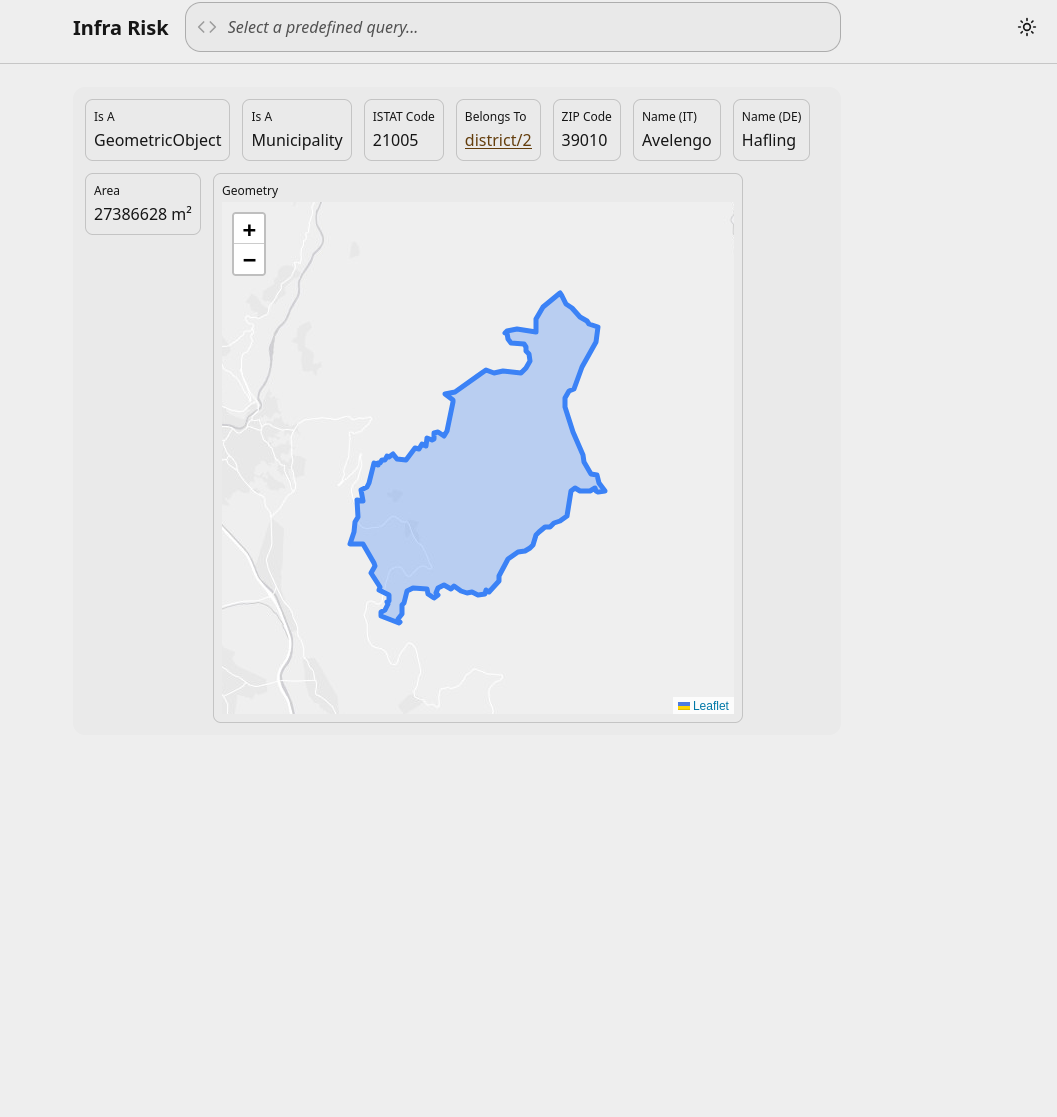
\includegraphics[width=\linewidth]{figures/municipality.png}
        \caption{Screenshot of the application showing the details for a single municipality.}
        \label{fig:municipality}
    \end{subfigure}
    \hfill
    \caption{Example screenshot extracted from the application showing the dedicated pages related to individual entities.}
    \label{fig:example3}
\end{figure}
